% Als je labels toe wilt voegen, doe het dan consequent
% voor een section ---> \label{sec:name_of_block}
%voor een subsection ---> \label{ssec:name_of_subsec}
%voor een subsubsec --> \label{sssec:name_of_subsubsec} en zo door

%Template voor elk apart blok EPO3 A4
\documentclass{scrartcl} % scrartcl of scrreprt
% Include all project wide packages here.
\usepackage{fullpage}
\usepackage{polyglossia}
\setmainlanguage{dutch}
\usepackage{csquotes}
\usepackage{graphicx}
\usepackage{epstopdf}
\usepackage{pdfpages}
\usepackage{caption}
\usepackage[list=true]{subcaption}
\usepackage{float}
%\usepackage{mathtools}
\usepackage{standalone}
\usepackage{import}
\usepackage{tocloft}
\usepackage{wrapfig}
\usepackage{authblk}
\usepackage{array}
\usepackage{booktabs}
\usepackage[toc,page,title,titletoc]{appendix}
\usepackage{xunicode}
\usepackage{amsmath}
\usepackage{fontspec}
\usepackage{unicode-math}
\usepackage[
    backend=bibtexu,
	texencoding=utf8,
bibencoding=utf8,
    style=ieee,
    sortlocale=nl_NL,
    language=auto
]{biblatex}
\usepackage{listings}
\newcommand{\includecode}[3][c]{\lstinputlisting[caption=#2, escapechar=, style=#1]{#3}}
\newcommand{\superscript}[1]{\ensuremath{^{\textrm{#1}}}}
\newcommand{\subscript}[1]{\ensuremath{_{\textrm{#1}}}}


\newcommand{\chapternumber}{\thechapter}
\renewcommand{\appendixname}{Bijlage}
\renewcommand{\appendixtocname}{Bijlagen}
\renewcommand{\appendixpagename}{Bijlagen}

\usepackage[hidelinks]{hyperref} %<--------ALTIJD ALS LAATSTE
 
\renewcommand{\familydefault}{\sfdefault}

\setmainfont[Ligatures=TeX]{Myriad Pro}
\setmathfont{Asana Math}
\setmonofont{Lucida Console}

\usepackage{titlesec, blindtext, color}
\definecolor{gray75}{gray}{0.75}
\newcommand{\hsp}{\hspace{20pt}}
\titleformat{\chapter}[hang]{\Huge\bfseries}{\chapternumber\hsp\textcolor{gray75}{|}\hsp}{0pt}{\Huge\bfseries}
\renewcommand{\familydefault}{\sfdefault}
\renewcommand{\arraystretch}{1.2}
\setlength\parindent{0pt}

%For code listings
\definecolor{black}{rgb}{0,0,0}
\definecolor{browntags}{rgb}{0.65,0.1,0.1}
\definecolor{bluestrings}{rgb}{0,0,1}
\definecolor{graycomments}{rgb}{0.4,0.4,0.4}
\definecolor{redkeywords}{rgb}{1,0,0}
\definecolor{bluekeywords}{rgb}{0.13,0.13,0.8}
\definecolor{greencomments}{rgb}{0,0.5,0}
\definecolor{redstrings}{rgb}{0.9,0,0}
\definecolor{purpleidentifiers}{rgb}{0.01,0,0.01}


\lstdefinestyle{csharp}{
language=[Sharp]C,
showspaces=false,
showtabs=false,
breaklines=true,
showstringspaces=false,
breakatwhitespace=true,
escapeinside={(*@}{@*)},
columns=fullflexible,
commentstyle=\color{greencomments},
keywordstyle=\color{bluekeywords}\bfseries,
stringstyle=\color{redstrings},
identifierstyle=\color{purpleidentifiers},
basicstyle=\ttfamily\small}

\lstdefinestyle{c}{
language=C,
showspaces=false,
showtabs=false,
breaklines=true,
showstringspaces=false,
breakatwhitespace=true,
escapeinside={(*@}{@*)},
columns=fullflexible,
commentstyle=\color{greencomments},
keywordstyle=\color{bluekeywords}\bfseries,
stringstyle=\color{bluestrings},
identifierstyle=\color{purpleidentifiers}
}

\lstdefinestyle{vhdl}{
language=VHDL,
showspaces=false,
showtabs=false,
breaklines=true,
showstringspaces=false,
breakatwhitespace=true,
escapeinside={(*@}{@*)},
columns=fullflexible,
commentstyle=\color{greencomments},
keywordstyle=\color{bluekeywords}\bfseries,
stringstyle=\color{redstrings},
identifierstyle=\color{purpleidentifiers}
}

\lstdefinestyle{xaml}{
language=XML,
showspaces=false,
showtabs=false,
breaklines=true,
showstringspaces=false,
breakatwhitespace=true,
escapeinside={(*@}{@*)},
columns=fullflexible,
commentstyle=\color{greencomments},
keywordstyle=\color{redkeywords},
stringstyle=\color{bluestrings},
tagstyle=\color{browntags},
morestring=[b]",
  morecomment=[s]{<?}{?>},
  morekeywords={xmlns,version,typex:AsyncRecords,x:Arguments,x:Boolean,x:Byte,x:Char,x:Class,x:ClassAttributes,x:ClassModifier,x:Code,x:ConnectionId,x:Decimal,x:Double,x:FactoryMethod,x:FieldModifier,x:Int16,x:Int32,x:Int64,x:Key,x:Members,x:Name,x:Object,x:Property,x:Shared,x:Single,x:String,x:Subclass,x:SynchronousMode,x:TimeSpan,x:TypeArguments,x:Uid,x:Uri,x:XData,Grid.Column,Grid.ColumnSpan,Click,ClipToBounds,Content,DropDownOpened,FontSize,Foreground,Header,Height,HorizontalAlignment,HorizontalContentAlignment,IsCancel,IsDefault,IsEnabled,IsSelected,Margin,MinHeight,MinWidth,Padding,SnapsToDevicePixels,Target,TextWrapping,Title,VerticalAlignment,VerticalContentAlignment,Width,WindowStartupLocation,Binding,Mode,OneWay,xmlns:x}
}

%defaults
\lstset{
basicstyle=\ttfamily\small,
extendedchars=false,
numbers=left,
numberstyle=\ttfamily\tiny,
stepnumber=1,
tabsize=4,
numbersep=5pt
}


\author{}% <------fill in your name
\title{EPO3: Eindrapport - Draw-pixel}

\begin{document}
\section{Drawpixel} %<----- fill in section name
\label{sec:drawpixel} % <-----fill in lable name

% describe function of block
Drawpixel is het blok dat het tekenen van een pixel implementeert. Drawpixel ontvangt via de instructiedecoder std\_standard\_logic vectoren x , y en color van de CPU. In de specificaties wordt ingegaan  op de lengte van deze vectoren. In het gedeelte daaronder wordt de verdere implementatie en het testen beschreven.

%specificaties blok (copy paste)
\subsection{Specificaties}
\label{ssec:specs_dp}
Door deze module worden aparte pixels getekend, hiervoor zijn de x- en y-coördinaten en de kleur van de pixel nodig. Drawpixel dient asb, y en x in een vector te plaatsen van lengte SizeRAMAddr, gedefinieerd in de package file. X en y zijn ook vectoren met lengten gedefinieerd in de package. Ook dient de color vector naar ramdata geschreven te worden.  Er moet alleen bij enable \& draw\_can\_access = hoog naar RAM geschreven worden, waarbij draw\_write gedurende het schrijven hoog is. (voor de controller)  Nadat er geschreven is, moet done gedurende een klokslag hoog worden. Er mag alleen in het niet actieve RAM geschreven worden, dus wanneer asb '0' is. Het hele blok met zijn in- en uitgangen is te zien in figuur  \ref{fig:dp_blokschema}. 
\begin{figure} [h!]
\centering
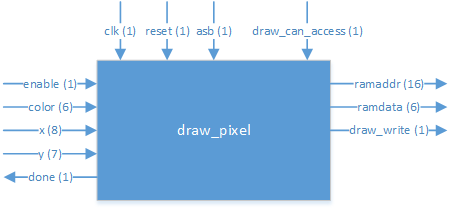
\includegraphics [width = \textwidth] {resource/dp_blokschema-rc}
\caption{Blokschema drawpixel}
\label{fig:dp_blokschema}
\end{figure}

%VHDL
\subsection{Ontwerp en specificatie}
\label{ssec:vhdl_dp}
\subsubsection{VHDL-Entity}
De entity is precies opgebouwd volgens  figuur  \ref{fig:dp_blokschema}. De in- en uitgangen zijn letterlijk overgenomen en zijn schaalbaar, zoals te zien in de figuur. Wanneer het vectoren betreft, die in de package omschreven worden, zijn het allemaal std\_logic\_vectoren. 

\subsubsection{VHDL-Behaviour}
De behaviour is opgedeeld in een sequentieel gedeelte waar de state 'busy' wordt opgeslagen en een combinatorisch gedeelte waar de signalen oe, draw\_write, done en de state worden bepaald. Oe is een tussensignaal op basis waarvan bepaald wordt of ramaddr en ramdata geschreven worden. Het is belangrijk dat de uitgangen 'Z' worden indien oe = 1 niet klopt, omdat de draad waarop de uitgang gezet wordt een bidirectional bus is. Het sequentiele process wordt getriggered op de clk, het combinatorische process op een verandering in reset, enable, draw\_can\_access of busy. 

%Testplan VHDL
\subsection{VHDL-simulatie}
\subsubsection{Test 1}
De eerste test betreft het simuleren van de behaviour met een testbench. Dit betreft een lege entity en een behaviour waarin een x-vector, y-vector en color-vector aangeboden worden volgens de lengte in de package file.  Er is ingezoomd op een gedeelte van de wave, namelijk wanneer er geschreven wordt naar het RAM

\begin{figure} [h!]
\centering
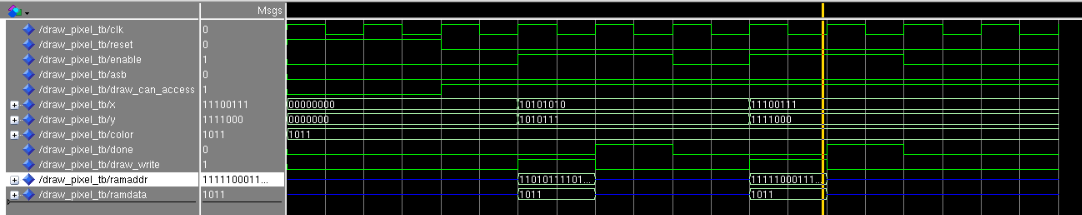
\includegraphics [scale = 0.7] {resource/dp_sim}
\caption{Modelsim simulatie behavioural of drawpixel}
\label{fig:dp_sim}
\end{figure}
\subsubsection{Test 2}
De tweede test betreft het testen van de synthesized VHDL. Op enkele begincondities na is deze gelijk aan  figuur \ref{fig:dp_sim}. 

\subsubsection{Test 3}
Om nog een extra test uit te voeren kan er uit de layout VHDL geëxtraheerd worden. Wanneer die vervolgens gesimuleerd wordt met modelsim, is te controleren of de schakeling op layoutniveau net zo werkt als op VHDL-niveau. Deze is exact gelijk aan test 2. 
%Synthese
\subsection{Synthese}
De synthese is nu uitgevoerd voor 6-bit kleur. 


%Switchlevel test
\subsection{Switchlevel}
Op switchlevel niveau wordt de simulatie op transistor niveau vergeleken met de simulatie op vhdl niveau. Hierbij wordt er vanuit de list-file een command file gemaakt. Vervolgens wordt via layout\ simulate en show\_result een simulatie geopend. Nu kan figuur \ref{fig:dp_sim} hiermee op het oog vergeleken worden. De optie compare geeft de mogelijkheid om dit exact te doen met GoWithTheFlow. De ref-file van de simulatie in figuur \ref{fig:dp_sim} wordt dan vergeleken met de res-file van de switch level simulatie. Is de implementatie goed dan horen alle waardes overeen te komen, op de eerste na. In ons ontwerp bevinden zich echter 'Z'-uitgangen, die door de compare niet goed begrepen worden. De noodzaak van 'Z's is al toegelicht. Het switch level resultaat komt overeen met het modelsim resultaat. 





%Conclusie
\subsection{Conclusie}
Alles was al gesimuleerd, gesynthetiseerd en getest toen bleek dat er meerdere pinnen voor de klok nodig zijn. Daardoor moest de kleur naar 3 bits. Nadat dat ook weer gesimuleerd, gesynthetiseerd en getest was bleek er ergens een fout te zitten, waardoor sprites niet werken. Pas als deze eruitgehaald is, en de nieuwe lengte van de color-vector bekend is, kan er weer gesynthetiseerd worden. Tot zover is dit verslag ook geschreven. 






\end{document}
